% ---------------------------------------------------------------------------
% Hornscope sample paper -- Applied Physics Letters (AIP REVTeX 4.2) format.
%
% Draft written from the analysis in this repository; every number in the
% tables and figures is produced by make_figures.py (see results.json).
% Items we do not yet know are marked \todo{...} and print in red.
%
% On Overleaf: Menu -> Main document -> sample_paper/main.tex
% ---------------------------------------------------------------------------
\documentclass[aip,apl,reprint,amsmath,amssymb]{revtex4-2}

\usepackage{graphicx}
\usepackage{xcolor}
\usepackage{tikz}
\usetikzlibrary{positioning}
\usepackage[colorlinks=true,linkcolor=blue,citecolor=blue,urlcolor=blue]{hyperref}

% Figures live in sample_paper/figures; the second path covers compiling from the repo root.
\graphicspath{{figures/}{sample_paper/figures/}}

\newcommand{\todo}[1]{\textcolor{red}{[TODO: #1]}}
\newcommand{\kms}{km\,s$^{-1}$}
\newcommand{\vlsr}{V_\mathrm{LSR}}

\begin{document}

\title{Galactic rotation and spiral structure from the 21\,cm hydrogen line with a low-cost foil-lined horn telescope}

\author{Davendra Hassan}
\author{Matt Sung}
\author{\todo{other team members}}
\affiliation{Department of Physics, National University of Singapore, Singapore}

\date{\today}

\begin{abstract}
We describe Hornscope, a pyramidal horn radio telescope built from acrylic sheets lined with aluminium foil, with a 3D-printed waveguide, a commercial low-noise amplifier and a USRP B200mini software-defined radio, developed for the PC5214 experimental physics course at the National University of Singapore. In four 5-minute pointings toward the Galactic plane we detect neutral hydrogen (HI) emission at signal-to-noise ratios of 10--14 per 1.17\,kHz channel (17--41 after smoothing to $\sim$7\,\kms). Line profiles toward the inner Galaxy are redshifted and those toward $\ell = 95^\circ$ blueshifted, as expected from differential Galactic rotation. Using the tangent-point method we obtain rotation speeds of $256$--$273$\,\kms\ at $R = 6.6$\,kpc and $210$--$229$\,\kms\ at $R = 5.2$\,kpc, consistent with previous small-telescope measurements. Kinematic distances place an HI component toward $\ell = 95^\circ$ on the Perseus arm. We discuss the instrumental effects that limit the measurement, notably the SDR's DC spike and the $\sim$20$^\circ$ beam.
\end{abstract}

\maketitle

% ===========================================================================
\section{Introduction}

The 21\,cm hyperfine transition of neutral hydrogen (HI) at $\nu_0 = 1420.405751$\,MHz was first detected in 1951\cite{EwenPurcell1951} and soon used to map the rotation and spiral structure of the Milky Way.\cite{vandeHulst1954,Oort1958} Because the line is intrinsically narrow and the interstellar medium is transparent at this wavelength, the Doppler shift of HI emission traces gas motions across the Galactic disk, including regions obscured at optical wavelengths.

The same measurement is now accessible to small teaching telescopes. Programs such as DSPIRA\cite{DSPIRA} have popularised pyramidal horn antennas combined with inexpensive software-defined radios (SDRs), and several groups have derived Galactic rotation curves with such instruments.\cite{Bhattacharjee2026,Liu2008,PhysicsOpenLab2020} Here we report the construction and first results of Hornscope, a horn telescope built with low-cost materials (acrylic, aluminium foil and 3D-printed parts) as a course project. We describe the instrument, the calibration and data reduction, the detection of HI in four directions, and the resulting rotation-curve and spiral-arm measurements, with emphasis on the instrumental effects that limit them.

% ===========================================================================
\section{Instrument}

\begin{figure}[t]
\centering
\resizebox{\columnwidth}{!}{%
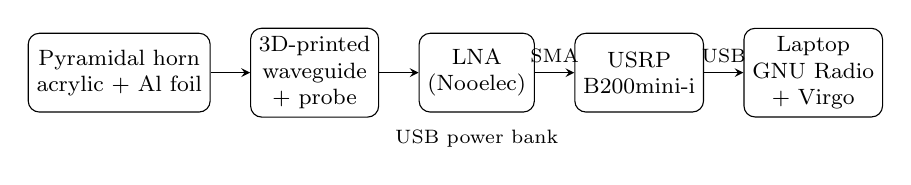
\begin{tikzpicture}[node distance=5mm, >=stealth,
  box/.style={draw, rounded corners, align=center, font=\footnotesize, minimum height=10mm, inner sep=3pt}]
  \node[box] (horn) {Pyramidal horn\\acrylic + Al foil};
  \node[box, right=of horn] (wg) {3D-printed\\waveguide\\+ probe};
  \node[box, right=of wg] (lna) {LNA\\(Nooelec)};
  \node[box, right=of lna] (sdr) {USRP\\B200mini-i};
  \node[box, right=of sdr] (pc) {Laptop\\GNU Radio\\+ Virgo};
  \draw[->] (horn) -- (wg);
  \draw[->] (wg) -- (lna);
  \draw[->] (lna) -- node[above, font=\scriptsize]{SMA} (sdr);
  \draw[->] (sdr) -- node[above, font=\scriptsize]{USB} (pc);
  \node[below=1mm of lna, font=\scriptsize] {USB power bank};
\end{tikzpicture}}
\caption{Hornscope signal chain. \todo{add a photograph of the horn and feed as panel (b).}}
\label{fig:chain}
\end{figure}

\textit{Antenna.} The horn follows the DSPIRA pyramidal geometry.\cite{DSPIRA,Bhattacharjee2026} Instead of laser-cut stainless steel, its walls are acrylic sheets lined with aluminium foil. The aperture is \todo{width $\times$ height} and the flare length \todo{length}. For reference, the stainless-steel DSPIRA horn of Ref.~\onlinecite{Bhattacharjee2026} (75\,cm $\times$ 60\,cm aperture) has a simulated gain of 18.5\,dBi and half-power beam widths of 18.1$^\circ$ and 21.3$^\circ$ in the E- and H-planes; we adopt a beam of $\sim$20$^\circ$ for Hornscope. \todo{measure the beam, e.g. with a solar drift scan.}

\textit{Feed.} The rectangular waveguide is 3D printed \todo{material, internal dimensions} and conductively lined with \todo{lining}. A quarter-wave monopole probe ($\lambda/4 \approx 5.3$\,cm at 1420\,MHz) \todo{confirm length and position} couples the waveguide mode to an SMA connector.

\textit{Receiver.} The probe output is amplified by a Nooelec low-noise amplifier \todo{model, e.g.\ SAWbird+ H1, and its gain/noise figure}, powered from a USB power bank, and digitised by an Ettus Research USRP B200mini-i (12-bit, UHD 4.9 driver) at 2.4\,MS/s centred on 1420.0\,MHz with 30\,dB of SDR gain. The SDR was connected over USB~2.0.

\textit{Software.} Spectra were recorded with Virgo,\cite{Virgo} a GNU Radio based spectrometer, using its weighted overlap-add (WOLA) channeliser with 2048 channels (1.17\,kHz, or 0.25\,\kms, per channel) and 1\,s integrations. Two issues in Virgo 3.8.2 were patched: it set the SDR's analog bandwidth to zero, which the B200mini interprets as its narrowest ($\sim$200\,kHz) filter and which removed the HI line from the band, and a plotting call incompatible with current matplotlib.

% ===========================================================================
\section{Observations and calibration}

Observations were made on 23 October 2026 from the NUS campus (1.30$^\circ$\,N, 103.78$^\circ$\,E). The horn was pointed manually, and the azimuth and altitude of each pointing were recorded (Table~\ref{tab:obs}). A 2-minute reference spectrum with the horn pointed at the ground was recorded first, followed by four 5-minute observations of the Galactic plane. Galactic coordinates were computed from the pointing and the mid-time of each recording.

\textit{Antenna check.} Pointing at the warm ground ($\sim$300\,K) should give more power than pointing at the sky. The ratio of sky to ground power, measured over line-free channels, was 0.65--0.76 (Table~\ref{tab:obs}), confirming that the antenna couples sky radiation into the receiver. During commissioning this test failed until we found that the LNA was unpowered; an unpowered LNA strongly attenuates the signal rather than passing it. Treating the ground as a 300\,K load and the sky as $\sim$10--30\,K, these ratios imply an effective system temperature of several hundred kelvin, an order of magnitude above the $\sim$60\,K reported for the steel horn of Ref.~\onlinecite{Bhattacharjee2026}. The ground is an imperfect load (the horn's sidelobes still see the sky), which biases this estimate high, but losses in the foil-lined horn and printed waveguide are also likely. \todo{repeat with a proper hot/cold calibration.}

\textit{Spectral calibration.} Each target spectrum was divided by the ground reference to remove the receiver bandpass, and a linear baseline fitted to line-free windows (1419.4--1419.9 and 1420.75--1420.95\,MHz) was removed, giving the fractional excess over the reference. Channels within $\pm$40\,kHz of the band centre, where the SDR's DC spike lies, were masked. For display and edge measurements, profiles were median-filtered over 9 channels and smoothed with a 25-channel boxcar ($\sim$7\,\kms\ resolution). Noise was estimated with a median absolute deviation in the line-free region 1419.4--1419.9\,MHz.

\textit{Velocities.} Frequencies were converted to radio velocities, $v = c(\nu_0 - \nu)/\nu_0$, and corrected to the local standard of rest (LSR) using the barycentric correction for each pointing and time plus the solar motion of Sch\"onrich \textit{et al.}\cite{Schoenrich2010} The corrections are listed in Table~\ref{tab:obs}.

\begin{table}[t]
\caption{Observations. All recordings are 5\,min with the ground reference \texttt{ground1}. $\Delta v$ is the LSR correction; $P/P_g$ the sky-to-ground power ratio; S/N is given per 1.17\,kHz channel and after smoothing to $\sim$7\,\kms.}
\label{tab:obs}
\begin{ruledtabular}
\begin{tabular}{lcccccccc}
 & Time & Az/Alt & $\ell$ & $b$ & $\Delta v$ & Peak $\vlsr$ & S/N & $P/P_g$ \\
 & (UTC+8) & (deg) & (deg) & (deg) & (\kms) & (\kms) & ch / sm & \\
\hline
mw1 & 15:36 & 65/45  & 53.4 & $+0.2$  & $-6.3$  & $+2.0$ & 13 / 41 & 0.74 \\
mw2 & 15:48 & 90/48  & 39.3 & $-10.3$ & $-12.6$ & $+3.3$ & 12 / 41 & 0.71 \\
mw3 & 16:05 & 33/17  & 94.7 & $+3.1$  & $+4.3$  & $-0.6$ & 10 / 25 & 0.76 \\
mw4 & 16:25 & 160/60 & 4.9  & $-4.1$  & $-14.8$ & $-1.7$ & 14 / 17 & 0.65 \\
\end{tabular}
\end{ruledtabular}
\end{table}

% ===========================================================================
\section{HI detections}

\begin{figure}[t]
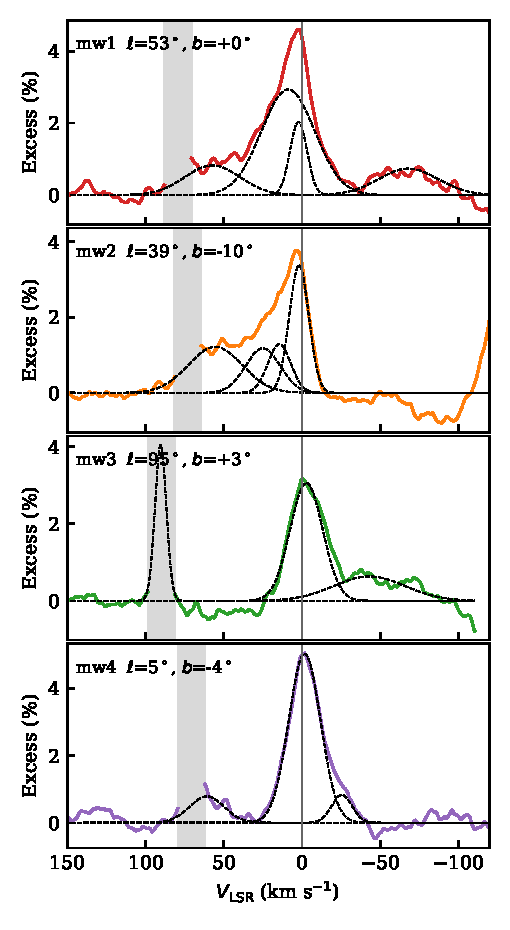
\includegraphics[width=\columnwidth]{fig_profiles}
\caption{HI profiles toward the four pointings, as fractional excess over the ground reference versus LSR velocity (smoothed to $\sim$7\,\kms). Dashed curves are the fitted Gaussian components (Table~\ref{tab:comp}). The grey band marks the channels masked around the SDR's DC spike. The rise at the right edge of mw2 is a band-edge artifact.}
\label{fig:profiles}
\end{figure}

HI emission is detected in all four directions (Fig.~\ref{fig:profiles}), with peak excesses of 3--5\% over the reference and signal-to-noise ratios of 10--14 per channel. The profiles differ systematically with longitude. Toward the inner Galaxy ($\ell = 5^\circ$, 39$^\circ$, 53$^\circ$) the emission peaks near $\vlsr \approx 0$ and extends to positive (redshifted) velocities, reaching the edge of the DC-spike mask at $\sim$70\,\kms. Toward $\ell = 95^\circ$ the emission extends instead to negative velocities, down to about $-60$\,\kms. Both are the signatures of differential Galactic rotation: inside the solar circle, gas along the line of sight recedes from the Sun, while beyond it, gas lags behind and appears to approach.

\begin{figure}[t]
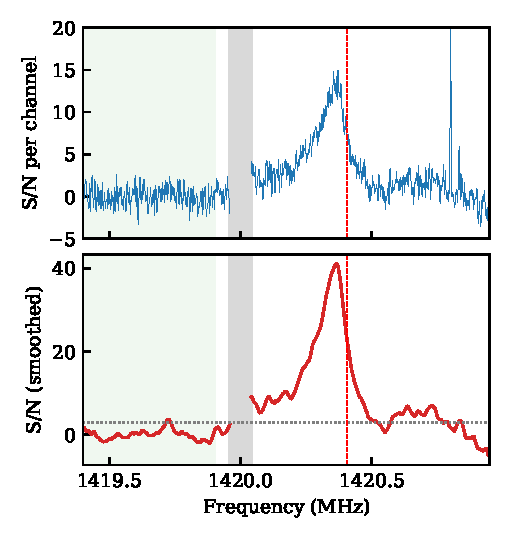
\includegraphics[width=\columnwidth]{fig_snr}
\caption{mw1 in individual 1.17\,kHz channels (top) and smoothed to $\sim$7\,\kms\ (bottom), each normalised by the noise in the shaded line-free region. The dashed line marks the HI rest frequency; the narrow spike near 1420.8\,MHz is radio-frequency interference.}
\label{fig:snr}
\end{figure}

The significance is illustrated for mw1 in Fig.~\ref{fig:snr}: the line is visible in single channels at S/N$\,\approx 13$, and smoothing to a resolution still well below the line width raises this to $\approx 41$. We note that the signal-to-noise panel produced by Virgo itself gives values $\sim$10 times lower, because its noise estimate includes the channels around the DC spike.

% ===========================================================================
\section{Rotation curve}

For a line of sight at $0^\circ < \ell < 90^\circ$, gas in circular orbits reaches its maximum (terminal) velocity at the tangent point, at Galactocentric radius
\begin{equation}
R = R_0 \sin\ell, \qquad V(R) = v_t + V_0 \sin\ell,
\label{eq:tangent}
\end{equation}
where $v_t$ is the terminal LSR velocity and we adopt $R_0 = 8.2$\,kpc and $V_0 = 230$\,\kms. We take $v_t$ where the smoothed profile falls below three times the noise. For mw1 and mw2 the profile is still well above this level where the DC-spike mask begins, so $v_t$ lies within the masked interval; we therefore quote the full range (Table~\ref{tab:rot}). The vertical error bars in Fig.~\ref{fig:rot} span this range plus an estimated $\pm$10\,\kms\ systematic uncertainty (baseline, reference drift and the adopted constants), and the horizontal bars correspond to $\pm$10$^\circ$ in $\ell$, the half-width of the beam.

\begin{table}[t]
\caption{Tangent-point analysis (Eq.~\ref{eq:tangent}). For mw1 and mw2 the terminal velocity $v_t$ lies within the DC-spike mask.}
\label{tab:rot}
\begin{ruledtabular}
\begin{tabular}{lcccc}
 & $\ell$ (deg) & $R$ (kpc) & $v_t$ (\kms) & $V$ (\kms) \\
\hline
mw1 & 53.4 & 6.59 & 71--88 & 256--273 \\
mw2 & 39.3 & 5.20 & 65--83 & 210--229 \\
mw4 & 4.9  & 0.70 & 18     & 37 \\
mw3\footnotemark[1] & 94.7 & 8.17 & 17 & 246 \\
\end{tabular}
\end{ruledtabular}
\footnotetext[1]{$\ell > 90^\circ$: no tangent point exists, and $V$ is dominated by the adopted $V_0$.}
\end{table}

\begin{figure}[t]
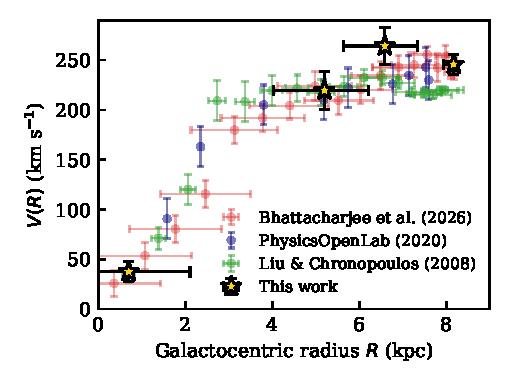
\includegraphics[width=\columnwidth]{fig_rotation}
\caption{Rotation-curve points from this work (stars) compared with previous small-telescope measurements: Bhattacharjee \textit{et al.}\cite{Bhattacharjee2026} (digitized from their figure), PhysicsOpenLab\cite{PhysicsOpenLab2020} and Liu \& Chronopoulos.\cite{Liu2008} The comparison studies use their published Galactic constants ($R_0 = 7.6$ and 7.97\,kpc, $V_0 = 220$\,\kms\ for the latter two).}
\label{fig:rot}
\end{figure}

The two pointings on or near the Galactic plane in the inner Galaxy give $V = 256$--273\,\kms\ at $R = 6.6$\,kpc (mw1) and $V = 210$--229\,\kms\ at $R = 5.2$\,kpc (mw2), in agreement with the earlier small-telescope results (Fig.~\ref{fig:rot}) and with the $\sim$220--240\,\kms\ found by large surveys at these radii.\cite{Sofue2009,Reid2014} mw1 lies slightly above the literature points; its upper range comes from the DC-spike mask, and a wide beam also tends to bias $v_t$ upward, because the terminal velocity is set by the part of the beam with the largest projected velocity. Although mw2 is centred 10$^\circ$ below the plane, its beam still reaches the plane, and it detects gas out to the mask.

The point at $R = 0.7$\,kpc (mw4) agrees with the steep inner rise found by the other small-telescope studies, but is far below the $\sim$200--250\,\kms\ measured in this region with higher angular resolution.\cite{Sofue2009} At small $\ell$ the 20$^\circ$ beam averages gas on both sides of the Galactic centre, the HI at the tangent points is sparse (much of the gas there is molecular), and gas in the Galactic bar does not follow circular orbits. The terminal velocity is then underestimated and Eq.~(\ref{eq:tangent}) reduces to $V \approx V_0 \sin\ell \propto R$, which explains the near-linear inner rise common to all the small-telescope curves. For mw3 ($\ell = 95^\circ$) there is no tangent point; its formal value is close to $V_0$ by construction and is shown for completeness only.

% ===========================================================================
\section{Spiral structure}

\begin{table}[t]
\caption{Gaussian components of the HI profiles and their kinematic distances $d$ for a flat rotation curve. Where two values are given, the near/far ambiguity is unresolved; ``tan'' marks components beyond the terminal velocity, placed at the tangent point.}
\label{tab:comp}
\begin{ruledtabular}
\begin{tabular}{lcccc}
 & $\vlsr$ (\kms) & $\sigma_v$ (\kms) & Amp.\ (\%) & $d$ (kpc) \\
\hline
mw1 & $-68.0 \pm 1.4$ & 18.9 & 0.74 & 16.1 \\
    & $+2.3 \pm 0.3$  & 5.4  & 2.04 & 0.2 / 9.6 \\
    & $+8.9 \pm 1.2$  & 17.0 & 2.94 & 0.7 / 9.1 \\
    & $+57.4 \pm 3.4$ & 17.5 & 0.83 & 4.9 (tan) \\
mw2 & $+1.9 \pm 3.6$  & 6.2  & 3.37 & 0.1 / 12.5 \\
    & $+14.5 \pm 9.9$ & 7.3  & 1.28 & 1.0 / 11.7 \\
    & $+25 \pm 100$   & 11.0 & 1.18 & 1.7 / 11.0 \\
    & $+55.6 \pm 19.3$& 17.2 & 1.22 & 3.5 / 9.2 \\
mw3 & $-43.0 \pm 2.8$ & 22.8 & 0.63 & 5.2 \\
    & $-2.8 \pm 0.3$  & 10.4 & 3.05 & 0.8 \\
    & $+90.4 \pm 0.9$\footnotemark[1] & 3.6 & 4.03 & --- \\
mw4 & $-25.4 \pm 3.7$ & 6.5  & 0.83 & 8.2 (tan) \\
    & $-1.6 \pm 0.8$  & 10.1 & 5.03 & 17.1 \\
    & $+60.9 \pm 6.1$ & 11.1 & 0.78 & 6.3 / 10.0 \\
\end{tabular}
\end{ruledtabular}
\footnotetext[1]{At the edge of the DC-spike mask; almost certainly an artifact. No kinematic solution exists for this velocity at $\ell = 95^\circ$.}
\end{table}

\begin{figure}[t]
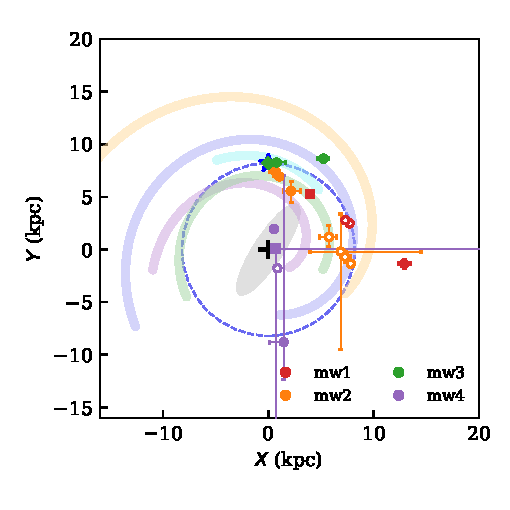
\includegraphics[width=\columnwidth]{fig_spiral}
\caption{HI components placed on the Galactic plane using kinematic distances (Sun at $Y = 8.2$\,kpc, Galactic centre at the origin, dashed circle: solar circle). Filled symbols: near or unique distances; open: far distances; squares: components placed at the tangent point. Shaded curves are approximate logarithmic-spiral models of the major arms\cite{Reid2014} (outward from the centre: Scutum--Centaurus, Sagittarius--Carina, Local, Perseus, Outer); the grey ellipse indicates the bar.}
\label{fig:spiral}
\end{figure}

Each profile was decomposed into up to four Gaussian components, with the number chosen by the Bayesian information criterion (Table~\ref{tab:comp}). Assuming a flat rotation curve, $v = V_0 \sin\ell\,(R_0/R - 1)\cos b$, each component velocity gives a Galactocentric radius $R$ and heliocentric distances $d = R_0\cos\ell \pm \sqrt{R^2 - R_0^2\sin^2\ell}$; both solutions are kept for the inner Galaxy, where they cannot be distinguished. Distance uncertainties propagate the fit error and a 5\,\kms\ allowance for random gas motions.

The resulting map (Fig.~\ref{fig:spiral}) is sparse but informative. The broad component at $-43$\,\kms\ toward $\ell = 95^\circ$ lies at $d \approx 5.2$\,kpc, on the Perseus arm. The tangent-point gas toward $\ell = 53^\circ$ and the near-side component at $+56$\,\kms\ toward $\ell = 39^\circ$ fall between the Sagittarius and Scutum arms, and several low-velocity components lie within 1\,kpc of the Sun. Some components are clearly unphysical or poorly constrained: the narrow $+90$\,\kms\ feature toward $\ell = 95^\circ$ sits at the edge of the DC-spike mask, the weak $-68$\,\kms\ component toward $\ell = 53^\circ$ may be baseline structure, and kinematic distances toward $\ell = 5^\circ$ are meaningless because the line of sight passes almost through the Galactic centre. With a $\sim$20$^\circ$ beam and only four directions, the map illustrates the method rather than resolving the arms.

% ===========================================================================
\section{Limitations and improvements}

The dominant limitation of the rotation-curve points is the SDR's DC spike, which falls at $\vlsr \approx +80$\,\kms\ when tuning to 1420.0\,MHz, exactly where inner-Galaxy terminal velocities lie. Tuning to 1420.9\,MHz would move it to $\approx -105$\,\kms. The $\sim$20$^\circ$ beam sets the horizontal error bars and biases terminal velocities. Our calibration is relative (signal-to-noise, not kelvin); a hot/cold calibration with a matched load would give brightness temperatures and a reliable system temperature. The ground reference drifted by up to $\sim$10\% over 5 minutes during warm-up and should be repeated every 30--60 minutes. A systematic survey along the plane at $\ell = 20^\circ$, 30$^\circ$, \dots, 80$^\circ$ would trace the curve from 2.8 to 8.1\,kpc.

% ===========================================================================
\section{Conclusion}

A horn telescope built from acrylic, aluminium foil and 3D-printed parts, with a commercial LNA and SDR, detects Galactic HI at high significance in 5-minute observations. The line profiles show the redshift--blueshift pattern of differential rotation, two pointings give rotation speeds of $\sim$210--270\,\kms\ at 5--7\,kpc in agreement with previous small-telescope work, and kinematic distances place one HI component on the Perseus arm. The main lessons for similar instruments are to verify that every active component in the signal chain is powered, to check the SDR's analog bandwidth, to keep the DC spike away from the velocities of interest, and to estimate noise away from it.

\begin{acknowledgments}
We thank \todo{PC5214 instructors and teaching assistants}. This work used GNU Radio, UHD, Virgo, Astropy, NumPy, SciPy and Matplotlib.
\end{acknowledgments}

\section*{Data availability}
The recordings, analysis scripts and figures are available at \url{https://github.com/verasha/hornscope}.

% ---------------------------------------------------------------------------
\begin{thebibliography}{99}

\bibitem{EwenPurcell1951}
H.~I. Ewen and E.~M. Purcell, ``Observation of a line in the Galactic radio spectrum,'' Nature \textbf{168}, 356 (1951).

\bibitem{vandeHulst1954}
H.~C. van de Hulst, C.~A. Muller, and J.~H. Oort, ``The spiral structure of the outer part of the Galactic system derived from the hydrogen emission at 21 cm wavelength,'' Bull. Astron. Inst. Netherlands \textbf{12}, 117 (1954).

\bibitem{Oort1958}
J.~H. Oort, F.~J. Kerr, and G. Westerhout, ``The Galactic system as a spiral nebula,'' Mon. Not. R. Astron. Soc. \textbf{118}, 379 (1958).

\bibitem{DSPIRA}
Digital Signal Processing in Radio Astronomy (DSPIRA), West Virginia University, \url{https://wvurail.org/dspira-lessons/}.

\bibitem{Bhattacharjee2026}
K. Bhattacharjee, H. Grover, and P. Arumugam, ``Observations of the 21 cm HI line from the Milky Way galaxy using pyramidal horn radio telescope,'' J. Astrophys. Astron. \textbf{47}, 75 (2026), arXiv:2512.19262.

\bibitem{Liu2008}
L. Liu and C. Chronopoulos, ``The hydrogen 21-cm line and its applications to radio astrophysics,'' MIT Junior Lab (8.14) report (2008), \url{https://web.mit.edu/lululiu/Public/8.14/21cm/21cm.pdf}.

\bibitem{PhysicsOpenLab2020}
PhysicsOpenLab, ``Milky Way rotation curve'' (2020), \todo{exact title and URL}.

\bibitem{Virgo}
A. Spanakis-Misirlis, Virgo: an easy-to-use spectrometer and radiometer for radio astronomy, \url{https://github.com/0xCoto/Virgo}.

\bibitem{Schoenrich2010}
R. Sch\"onrich, J. Binney, and W. Dehnen, ``Local kinematics and the local standard of rest,'' Mon. Not. R. Astron. Soc. \textbf{403}, 1829 (2010).

\bibitem{Reid2014}
M.~J. Reid \textit{et al.}, ``Trigonometric parallaxes of high mass star forming regions: the structure and kinematics of the Milky Way,'' Astrophys. J. \textbf{783}, 130 (2014).

\bibitem{Sofue2009}
Y. Sofue, M. Honma, and T. Omodaka, ``Unified rotation curve of the Galaxy -- decomposition into de Vaucouleurs bulge, disk, dark halo, and the 9-kpc rotation dip,'' Publ. Astron. Soc. Jpn. \textbf{61}, 227 (2009).

\end{thebibliography}

\end{document}
